\documentclass[12pt]{article}
\usepackage[left=12mm, top=0.5in, bottom=0.5in]{geometry}
\usepackage{amsmath}
\usepackage{mathtools}
\usepackage{amssymb}
\usepackage{pifont}
\usepackage{tikz-qtree}
\usepackage{tikz}
\usetikzlibrary{trees}

\newcommand{\cmark}{\ding{51}}%
\newcommand{\xmark}{\ding{55}}%
\newcommand\tab[1][1cm]{\hspace*{#1}}

\begin{document}

\title{CS 440 Assignment \#3, Part 1}
\author{Austin Bennett}
\maketitle

\section *{Problem 1}
(a) $P(A = true, B = true, C = true, D = true, E = true) \\
 \Rightarrow P(A=t)* P(B=t)* P(C=t)* P(D=t | A=t, B=t)* P(E =t | B = t, C =t) \\
 \Rightarrow 0.2 * 0.5 * 0.8 * 0.1 * 0.3  \\
 \Rightarrow P(A = true, B = true, C = true, D = true, E = true) = 0.0024  \\ \\
(b) P(A = false, B = false, C = false, D = false, E = false) \\
 \Rightarrow P(A=f)* P(B=f)* P(C=f)* P(D=f | A=f, B=f)* P(E =f | B = f, C =f) \\
 \Rightarrow 0.8*0.5*0.2*0.9*0.2  \\
 \Rightarrow P(A = false, B = false, C = false, D = false, E = false) = 0.0144 $ \\ \\
(c) $P(A = true | B = false, C = false, D = false, E = false) \\
\Rightarrow P(A = t | B = f, C = f, D = f, E = f) \\
\Rightarrow P(A | B = f, C = f, D = f, E = f) \\
\Rightarrow \propto P(A, B = f, C = f, D = f, E = f) \\
\Rightarrow \propto \sum\limits_{B} \sum\limits_{C} P(A)*P(B)*P(C)*P(D| A, B)*P(E|B,C) \\
\Rightarrow \propto P(A) \sum\limits_{B} P(B) \sum\limits_{C} P(C)*P(D| A, B)*P(E|B,C)$ \\
\begin{gather} 
P(A=t) *  \sum\limits_{B} P(B) \sum\limits_{C} P(C)*P(D| A, B)*P(E|B,C) + \\
P(A = f) *  \sum\limits_{B} P(B) \sum\limits_{C} P(C)*P(D| A, B)*P(E|B,C)
\end{gather} \\
\begin{gather}
 P(A=t) * P(B=t) \sum\limits_{C} P(C)*P(D| A, B)*P(E|B,C) + \\
 P(A=t) * P(B=f) \sum\limits_{C} P(C)*P(D| A, B)*P(E|B,C)  \\
 P(A=f) * P(B=t) \sum\limits_{C} P(C)*P(D| A, B)*P(E|B,C) + \\
 P(A=f) * P(B=f) \sum\limits_{C} P(C)*P(D| A, B)*P(E|B,C)
\end{gather}\\
\begin{gather}
 P(A=t) * P(B=t)*P(C=t)*P(D| A, B)*P(E|B,C=t) + \\
 P(A=t) * P(B=t)*P(C=f)*P(D| A, B)*P(E|B,C=f)  + \\
 P(A=t) * P(B=f)*P(C=t)*P(D| A, B)*P(E|B,C=t)  + \\
 P(A=t) * P(B=f)*P(C=f)*P(D| A, B)*P(E|B,C=f)   \\
 P(A=f) * P(B=t)*P(C=t)*P(D| A, B)*P(E|B,C=t) + \\
 P(A=f) * P(B=t)*P(C=f)*P(D| A, B)*P(E|B,C=f) + \\
 P(A=f) * P(B=f)*P(C=t)*P(D| A, B)*P(E|B,C=t)  + \\
 P(A=f) * P(B=f)*P(C=f)*P(D| A, B)*P(E|B,C=f) 
\end{gather}\\
\begin{gather}
.2*.5*.8*.1*.3 + \\
.2*.5*.2*.1*.8 + \\
.2*.5*.8*.5*.4 + \\
.2*.5*.2*.5*.2 \\
.8*.5*.8*.6*.3 + \\
.8*.5*.2*.6*.8 + \\
.8*.5*.8*.9*.4 + \\
.8*.5*.2*.9*.2
\end{gather}\\
Let x = $P(A = t, B = f, C = f, D = f, E = f) = (15) + (16) + (17) + (18) = .0.022 $\\
Let y = $P(A = f, B = f, C = f, D = f, E = f) = (19) + (20) + (21) + (22) = .2256$\\
$\propto = \frac{1}{x+y} \approx 4$\\
$\propto P(A, B = f, C = f, D = f, E = f) = \{.088, .9024\}$ \\ 
Thus, $P(A = t | B = f, C = f, D = f, E = f) = .088 $\\ 
\newpage
\section *{Problem 2}
(a) $P(Burglary | JohnCalls = true, MaryCalls = true) \\
\Rightarrow P(B | J = t, M = t) \\
\Rightarrow P(B | J = t, M = t, A, E) \\
\Rightarrow \propto P(B, J = t, M = t, A, E) \\
\Rightarrow \propto \sum\limits_{E} \sum\limits_{A} P(B)*P(J|A)*P(M|A)*P(A|B, E)*P(E) \\
\Rightarrow \propto P(B) \sum\limits_{E} P(E) \sum\limits_{A} P(J|A) * P(M|A)*P(A|B, E)$ \\
\begin{gather} 
 P(B=t) * \sum\limits_{E} P(E) \sum\limits_{A} P(J|A) * P(M|A)*P(A|B, E) + \\
P(B = f) * \sum\limits_{E} P(E) \sum\limits_{A} P(J|A) * P(M|A)*P(A|B, E)
\end{gather} \\
\begin{gather}
 P(B=t) * P(E=t) \sum\limits_{A} P(J|A) * P(M|A)*P(A|B, E) + \\
 P(B=t) * P(E=f) \sum\limits_{A} P(J|A) * P(M|A)*P(A|B, E)  \\
 P(B=f) * P(E=t) \sum\limits_{A} P(J|A) * P(M|A)*P(A|B, E) + \\
 P(B=f) * P(E=f) \sum\limits_{A} P(J|A) * P(M|A)*P(A|B, E)
\end{gather}\\
\begin{gather}
 P(B=t) * P(E=t)* P(J|A=t) * P(M|A=t)*P(A=t|B, E) + \\
 P(B=t) * P(E=t)* P(J|A=f) * P(M|A=f)*P(A=f|B, E) + \\
 P(B=t) * P(E=f)* P(J|A=t) * P(M|A=t)*P(A=t|B, E) + \\
 P(B=t) * P(E=f)* P(J|A=f) * P(M|A=f)*P(A=f|B, E)  \\
 P(B=f) * P(E=t)* P(J|A=t) * P(M|A=t)*P(A=t|B, E) + \\
 P(B=f) * P(E=t)* P(J|A=f) * P(M|A=f)*P(A=f|B, E) + \\
 P(B=f) * P(E=f)* P(J|A=t) * P(M|A=t)*P(A=t|B, E) + \\
 P(B=f) * P(E=f)* P(J|A=f) * P(M|A=f)*P(A=f|B, E)
\end{gather}\\
\begin{gather}
.0001*.002*.9*.7*.95 + \\
.001*.002*.05*.01*.05 + \\
.001*.998*.9*.7*.94 + \\
.001*.998*.05*.01*.06  \\
.999*.002*.9*.7*.29 + \\
.999*.002*.05*.01*.71 + \\
.999*.998*.9*.7*.001 + \\
.999*.998*.05*.01*.999 
\end{gather}\\
Let x = $P(B=t, J = t, M = t, A, E) = (37) + (38) + (39) + (40) = .00059224 $\\
Let y = $P(B=f, J = t, M = t, A, E) = (41) + (42) + (43) + (44) = .0014919$\\
$\propto = \frac{1}{x+y} \approx 480$\\
$\propto P(B, J = t, M = t, A, E) = \{.284, .716\}$ \\ \\
(b) Given a sequence of Boolean variables $X_1$, \dots $X_n$ where Parents($X_i$) = $\{X_{i-1}\}$ for i = 2, \dots, n \\
To compute the complexity of $P(X_1|X_n = true)$ using enumeration, we first need to understand that $P(X_1|X_n = true) \equiv P(X_1, \dots, X_{n-1}, X_n = true)$ \\
So we have a bayesian distribution with n boolean variables and thus we have $2^n$ possible outcomes. For each of these $2^n$ possible outcomes we must compute n-1 multiplications and finally n-2 additions. \\
On top of these computations is our computation for $\propto$, which is based on prior calculations, thus is a mere 2 operations to compute and an additional operation to multiply over our probability distribution. \\
After removing constants we can deduce that the complexity of $P(X_1|X_n = true)$ using enumeration = $O(n^2 2^n)$ \\
Using variable elimination instead of enumeration, can we reduce the amount of work required for $P(X_1|X_n = true)$? \\ \\
Unforunately for us it does not take much time to realize that due to the fact that the entire bayesian network is connected such that $X_1$ is the parent of every variable in the network: every variable relies on their successors and as such their is no repition in the inference tree that is derived from the network. Thus, the complexity using variable elimination can not be improved over the enumeration method for this particular network.



\newpage
\section *{Problem 3}
(a)
\begin{figure}[!htb]
	\centering
	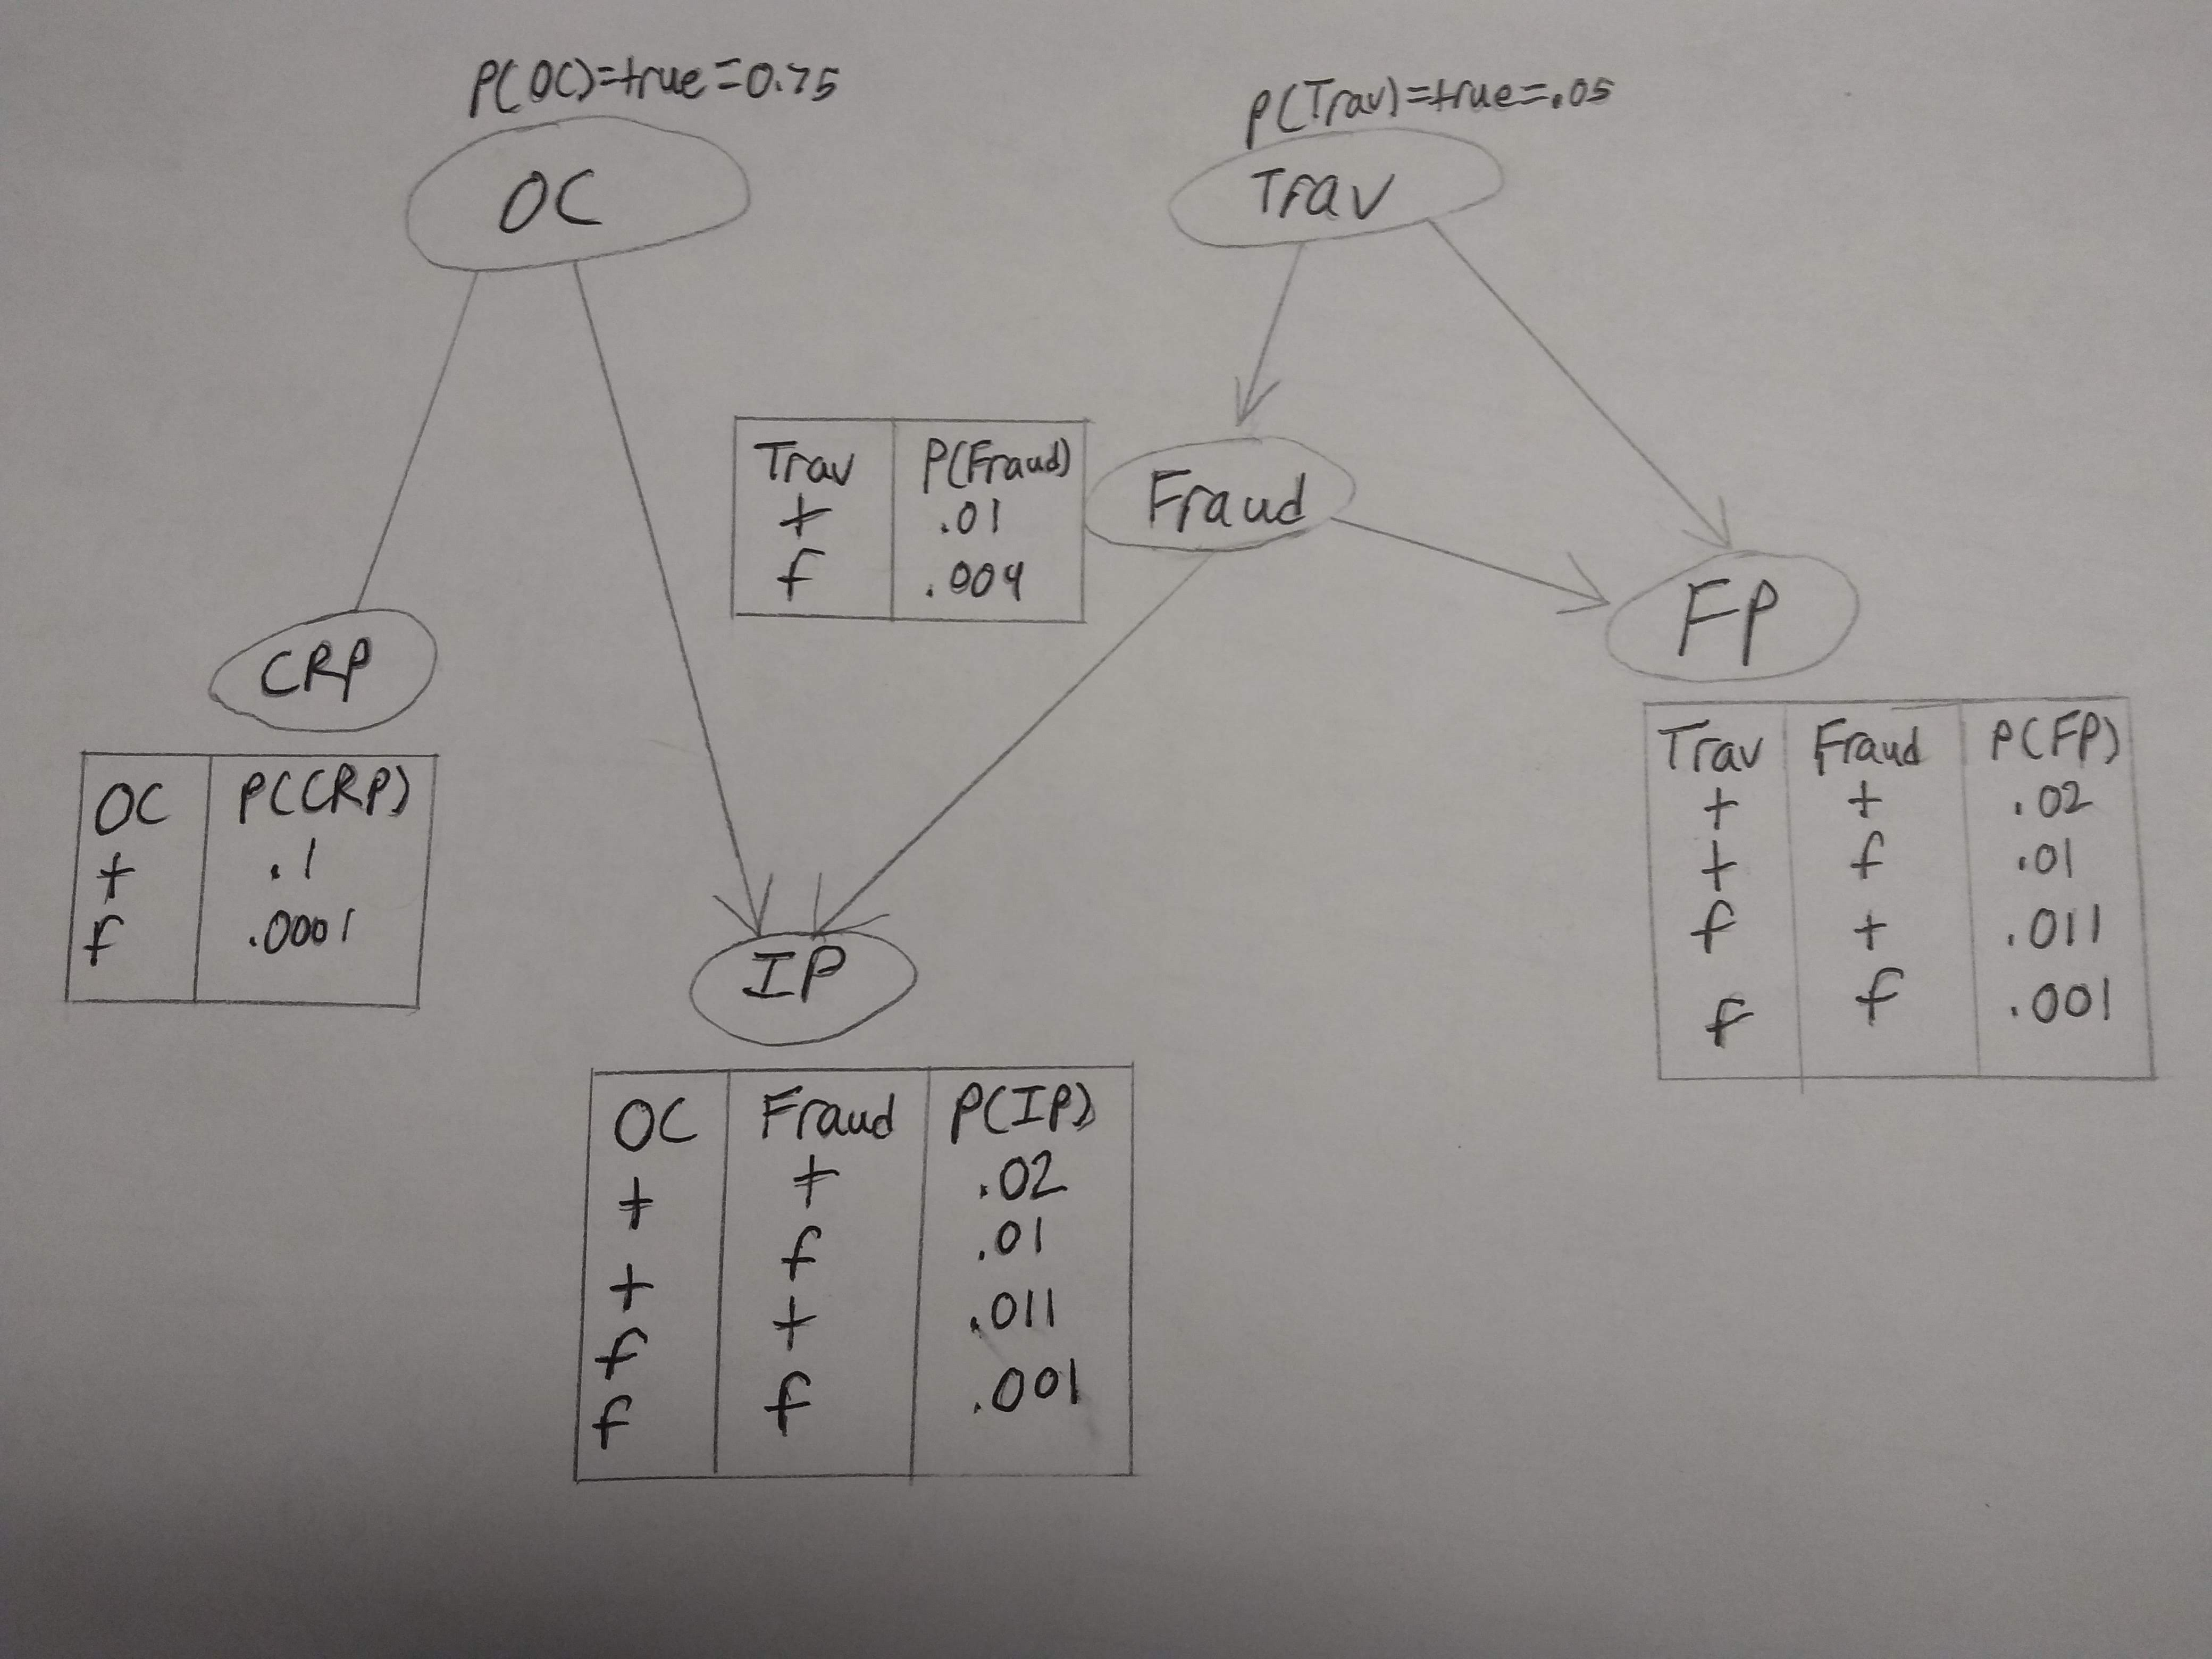
\includegraphics[width=.8\textwidth]{problem3_2.jpg}
\end{figure} \\ \\
(b) $P(Fraud | Trav) \\
\Rightarrow P(Fraud | Trav =t) + P(Fraud | Trav = f) \\
\Rightarrow P(Fraud | Trav =t)*P(Trav = t) + P(Fraud | Trav = f)*P(Trav =f) \\
\Rightarrow .01*.05 + .004*.95 = .0043 = P(Fraud | Trav) $ \\ \newpage
$P(Fraud | FP = true, IP = false, CRP = true) \\
\Rightarrow P(F | FP = t, IP = f, CRP = t) \\
\Rightarrow P(F | FP = t, IP = f, CRP = t, OC, T) \\
\Rightarrow \propto P(F, FP = t, IP = f, CRP = t, OC, T) \\
\Rightarrow \propto \sum\limits_{OC} \sum\limits_{T} P(F)*P(FP | T, F)*P(IP|OC, F)*P(CRP|OC) \\
\Rightarrow \propto P(F) \sum\limits_{T} P(FP|T, F) \sum\limits_{OC} P(IP|OC,F)*P(CRP|OC)$ \\
\begin{gather} 
 P(F= t) \sum\limits_{T} P(FP|T, F) \sum\limits_{OC} P(IP|OC,F)*P(CRP|OC) + \\
 P(F = f) \sum\limits_{T} P(FP|T, F) \sum\limits_{OC} P(IP|OC,F)*P(CRP|OC)
\end{gather} \\
\begin{gather}
 P(F= t)*P(FP|T = t, F) \sum\limits_{OC} P(IP|OC,F)*P(CRP|OC) + \\
 P(F= t)*P(FP|T = f, F) \sum\limits_{OC} P(IP|OC,F)*P(CRP|OC) \\
P(F= f)*P(FP|T = t, F) \sum\limits_{OC} P(IP|OC,F)*P(CRP|OC) + \\
 P(F= f)*P(FP|T = f, F) \sum\limits_{OC} P(IP|OC,F)*P(CRP|OC) \\
\end{gather}\\
\begin{gather}
 P(F= t)*P(FP|T = t, F)* P(IP|OC=t,F)*P(CRP|OC=t) + \\
 P(F= t)*P(FP|T = t, F)* P(IP|OC=f,F)*P(CRP|OC=f) + \\
 P(F= t)*P(FP|T = f, F)* P(IP|OC=t,F)*P(CRP|OC=t) + \\
 P(F= t)*P(FP|T = f, F)* P(IP|OC=f,F)*P(CRP|OC=f)  \\
 P(F= f)*P(FP|T = t, F)* P(IP|OC=t,F)*P(CRP|OC=t) + \\
 P(F= f)*P(FP|T = t, F)* P(IP|OC=f,F)*P(CRP|OC=f) + \\
 P(F= f)*P(FP|T = f, F)* P(IP|OC=t,F)*P(CRP|OC=t) + \\
 P(F= f)*P(FP|T = f, F)* P(IP|OC=f,F)*P(CRP|OC=f) 
\end{gather}\\
\begin{gather}
.0043*.02*.02*.1 + \\
.0043*.02*.011*.0001 + \\
.0043*.011*.02*.1 + \\
.0043*.011*.011*.0001 \\
.9957*.2*.02*.1 + \\
.9957*.2*.011*.0001 + \\
.9957*.011*.02*.1 + \\
.9957*.011*.011*.0001 
\end{gather}\\
Let x = $P(F = t, FP = t, IP = f, CRP = t, OC, T) = (60) + (61) + (62) + (63) =  .00000026675$\\
Let y = $P(F = f, FP = t, IP = f, CRP = t, OC, T) = (64) + (65) + (66) + (67) = .00042042$\\
$\propto = \frac{1}{x+y} \approx 2377$\\
$\propto P(F, FP = t, IP = f, CRP = t, OC, T) = \{.00063406,.99933\}$ \\ 
Good news! It is extremely unlikely the transaction was fraudulent.\\

\end{document}